\documentclass[twoside,fancyhdr]{18_format/csethesis}
%\documentclass{18_format/iitgthesis}
\pdfminorversion=7
\listfiles
\input{17_Util/usepackage}
\usepackage{pdfpages}
%\setlist[description]{style = multiline, labelwidth = 40pt}
%%%%%%%%%%%%%%%%%%%%%%%%%%%%%%%%%%%%%%%%%%%%%%%%%%%%%%%%%
%=============================================================================
% SEGREGATE THE BIBLIOGRAPHY
%=============================================================================
%\newcites{th}{Publications Related to Thesis}
%\newcites{gen}{Other Publications of the Author}
\addbibresource{20_bibilography/ref-article.bib}
\addbibresource{20_bibilography/ref-proc.bib}
\addbibresource{20_bibilography/ref-oth.bib}
%\addbibresource{20_bibilography/total6.bib}
%\addbibresource{20_bibilography/new.bib}
\addbibresource{20_bibilography/mypub.bib}
%%%%%%%%%%%%%%%%
\DeclareCiteCommand{\citenum}
  {}
  {\printfield{labelnumber}}
  {}
  {}
%%%%%%%%%%%%%%%%  
\defbibenvironment{mypubs}
  {\enumerate[label={[T.\arabic*]}]
     {}
     {\setlength{\labelwidth}{\labelnumberwidth}%
      \setlength{\leftmargin}{\labelwidth}%
      \setlength{\labelsep}{\biblabelsep}%
      \addtolength{\leftmargin}{\labelsep}%
      \setlength{\itemsep}{\bibitemsep}%
      \setlength{\parsep}{\bibparsep}}%
      \renewcommand*{\makelabel}[1]{\hss##1}}
  {\endenumerate}
  {\item}
%%%%%%%%%%%%%%%%
\defbibenvironment{mypuboth}
  {\enumerate[label={[O.\arabic*]}]
     {}
     {\setlength{\labelwidth}{\labelnumberwidth}%
      \setlength{\leftmargin}{\labelwidth}%
      \setlength{\labelsep}{\biblabelsep}%
      \addtolength{\leftmargin}{\labelsep}%
      \setlength{\itemsep}{\bibitemsep}%
      \setlength{\parsep}{\bibparsep}}%
      \renewcommand*{\makelabel}[1]{\hss##1}}
  {\endenumerate}
  {\item}
%%%%%%%%%%%%%%%%%%%%%%%%%%%%%%%%%%%%%%%%%%%%%%%%%%%%%%%%%
\input{17_Util/newcommands}
%%%%%%%%%%%%%%%%%%%%%%%%%%%%%%%%%%%%%%%%%%%%%%%%%%%%%%%%%
%\def\macro{Modular and Response}
%%%%%%%%%%%%%%%%%%%%%%%%%%%%%%%%%%%%%%%%%%%%%%%%%%%%%%%%%
%\linenumbers
%\usepackage{style/qtree}
%%%%%%%%%%%%%%%%%%%%%%%%%%%%%%%%%%%%%%%%%%%%%%%%%%%%%%%%%
\phdtitle = {{SDN for Large Scale IoT Networks}} % { and } are needed around your name
%\phdtitle = {{Light-weight Self-stabilizing Dynamic NIB Placement For Distributed Large Scale SDN}}
\name = {Subhrendu Chattopadhyay}          % and other fields. don't remove.
\rollno = {146101002}
\guide = {Prof. Sukumar Nandi}
%%%%%%%%%%%%%%%%%%%%%%%%%%%%%%%%%%%%%%%%%%%%%%%%%%%%%%%%%%%%%%%%%
\begin{document}
  %%%% Front Cover Page
  \pagenumbering{alph}
  \pdfbookmark{Front Cover}{Front Cover}
  %%============================================================================
%% FrontCoverPage
%%===========================================================================
%\pagenumbering{roman}
%%\chapter*{}
%\thispagestyle{empty}
%%\pagecolor{covercolor}
%\color{coverfont}
%\newgeometry{margin=0pt}
%%\pagecolor{covercolor} % Cover color defined in \17_Util/newcommands.tex
%%\begin{center}
%%\begin{overpic}[width=.99\paperwidth]{0-cover/ThesisTopCover.png}% add grid to options for positioning
%%Adjust title position by changing \put (x,y)
% %\put(0,0){A} \put(67,99){B}
%% \put (0,86){\transparent{0.8}\mycbox{black}{17cm}{3cm}} % background boxes
%% \put (4,90) {\begin{minipage}{0.7\linewidth} \huge\sf\textbf{\the\phdtitle}\end{minipage}}
%% \put (24,16){\transparent{0.8}\mycbox{black}{13cm}{3cm}} % background boxes
%% \put(29,21){{\LARGE{\textbf{\textit{\the\name}}}}}
%%\end{overpic} 
%%\end{center}
%%\cleardoublepage
%\pagecolor{white}
%%\cleardoublepage
%\color{black}
%\restoregeometry
%============================================================================
% FrontCoverPage
%===========================================================================
\pagenumbering{roman}
%\chapter*{}
\thispagestyle{empty}
\textheight 16in \textwidth 12.5in {\huge\sf  \textbf{\the\phdtitle}}\\[100ex]

\begin{flushright}
\LARGE{\textbf{\textit{\the\name}}}
\end{flushright}
%\cleardoublepage

%  \includepdf[pages={2}]{C0_Cover.pdf}
  %\linenumbers
    \clearpage  
  %\blankpage
  %\startOddPage
  \pagenumbering{roman}
  \pdfbookmark{Title Page}{Title Page}
  \newgeometry{margin=0pt}
\chapter*{}
\pagenumbering{roman}
\thispagestyle{empty}
%\begin{titlepage}
\begin{center}
%\textheight 5in \textwidth 12.5in {\huge\sf  \textbf{  }}\\[5ex]
\textheight 16in \textwidth 12.5in {\huge\sf  \textbf{\the\phdtitle}}\\[20ex]
{\Large{\textit{
%{\Large \bf Synopsis Report}\\
{Thesis submitted in partial fulfilment \\of the requirements
for the degree of\\
[5ex]{\Large \bf Doctor of Philosophy}
}}}}\\
[5ex] \large\emph{by} \\[1ex]
{\sf \sf \Large\bf{\the\name}}\\[5ex]
\large\textit{under the supervision of}\\[2ex]
{\Large \bf \the\guide} \\[5ex]

%\vspace{.05in}
 \begin{figure}
    \begin{minipage}{\linewidth}
      \centering
      
\includegraphics[scale=.9]{0-title/iitg_logo}
    \end{minipage} 
  \end{figure}

%{\sl \bf{to the}} \\[1ex]
{\large \bf Department of Computer Science and Engineering}  \\[1ex]
{\Large \bf{INDIAN INSTITUTE OF TECHNOLOGY GUWAHATI \\GUWAHATI - 781039, INDIA}}\\
{\large\bf {\today}}
\end{center}
\restoregeometry

  \startOddPage
  %\pagenumbering{roman}
\thispagestyle{plain}
\chapter*{}
  \pdfbookmark{Dedication}{Dedication}
\vskip 1.5cm
\dedication
    \begin{figure}[!ht]
        \centering
        \begin{minipage}{\textwidth}
            \centering
            \includegraphics[clip, trim=0 250 20 0, width=\textwidth]{0-certificate/Quote.pdf}
        \end{minipage}
    \end{figure}
    \textbf{\textit{\Large{``The absolute knowledge can be attained after thinking, reasoning and assimilation''}}} \\[10ex]
    \textbf{\textit{\Huge{Dedicated to}}}\\[3ex]
   \textbf{\textit{\Huge{All my teachers}}}\\[3ex]
   \normalsize{\it Who taught me to assimilate the information to convert it into knowledge.}
   \clearpage
\enddedication
%\startOddPage
%%%%%%%%%%%%%%%%%%%%%%%%%%%%%%%%%%%%%%%%%%%%%%%%%%%%%%%%%%%%%%%%%%%%%%%%%%%%%%%%%%%%
%\raggedbottom
%\thispagestyle{empty}
\chapter*{\centering Declaration}
  \pdfbookmark{Declarations}{Declarations}
%\begin{Declaration}
 I declare that
 \begin{enumerate}
  \item The work contained in this thesis is original and has been done by myself under the general supervision of my supervisor.
  \item The work has not been submitted to any other Institute for any degree or diploma.
  \item Whenever I have used materials (data, theoretical analysis, results) from other sources, I have given due credit to them by citing them in the text of the thesis and giving their details in the references.
  \item Whenever I have quoted written materials from other sources, I have put them under quotation marks and given due credit to the sources by citing them and giving required details in the references. 
 \end{enumerate}
\vspace{2cm}
%\begin{flushright}
\begin{tabular}{p{.3\textwidth}l}
Place: IIT Guwahati  &\large \textbf{Subhrendu Chattopadhyay}\\
Date:  & Research Scholar\\
  & Department of Computer Science and Engineering, \\
  & Indian Institute of Technology Guwahati,\\
  & Guwahati, INDIA 781039
\end{tabular}
%\end{flushright}
%\end{Declaration}
%%%%%%%%%%%%%%%%%%%%%%%%%%%%%%%%%%%%%%%%%%%%%%%%%%%%%%%%%%%%%%%
\startOddPage
\chapter*{\centering Certificate}
%\begin{Certificate}
  \pdfbookmark{Certificates}{Certificates}
\vskip 2ex \quad This is to certify that the work contained
in this thesis entitled ``\the\phdtitle'' 
is a bonafide work of \the\name
(Roll No. \the\rollno), carried out in the Department of
Computer Science and Engineering, Indian Institute of Technology
Guwahati under my supervision and that it has not been submitted
elsewhere for a degree.

\vspace{2cm}
\begin{tabular}{p{.3\textwidth}l}
Place: IIT Guwahati & \large \textbf{\the\guide}\\
Date:  &Department of Computer Science and Engineering, \\
 & Indian Institute of Technology Guwahati,\\
 & Guwahati, INDIA 781039
\end{tabular}
%\end{Certificate}
%\clearpage
\startOddPage
  \clearpage  
  %\startOddPage
  \chapter*{\centering Acknowledgements}
\addcontentsline{toc}{chapter}{Acknowledgements}
\thispagestyle{cleanPage}
This thesis would not have been complete without the support of my thesis supervisor \textit{Prof. Sukumar Nandi} and my mentor \textit{Dr. Sandip Chakraborty}. Both of them have provided their support, knowledge and guidance to help me in my research. I have been working with both of them from my early days of M.Tech. I am truly grateful to them for putting me back in track during the trying times of my PhD. I have also learned many things about life while having a discussion with them. Their constant support and positive criticism have influenced my attitude, nature and personality in many ways.

I am very thankful to my doctoral committee members \textit{Prof. Diganta Goswami}, \textit{Prof. Ratnajit Bhattacharya} and \textit{Dr. Tamarapalli Venkatesh} for understanding my works and providing valuable comments to improve the work. I express my sincere thanks to former \textit{Head of the Department} \textit{Prof. S.B. Nair} and \textit{Prof. S.V. Rao} and current \textit{Head of the Department} \textit{Prof. Jatindra Deka} for providing a nice research environment in the \textit{Department of Computer Science and Engineering, IITG} and support my research work in many ways. During my early stages of research I enjoyed discussion with \textit{Dr. Sushanta Karmakar} and \textit{Dr. Arnab Sarkar} who helped and motivated me in a lot of ways. I am forever grateful for their support and time.

I am also very grateful to \textit{Tata Consultancy Services India Private Limited} for awarding me the research fellowship that gave me extremely good opportunities to broaden my research activities and interact with eminent researchers in the world, both from the industry as well from the academia. I thank \textit{Mr. Sachin Parkhi}, \textit{Program Manager of TCS Research Scholar Program}, for extending their helps and supports in technical and official activities. 

I had the privilege to collaborate with \textit{Dr. Sushanta Karmakar}, \textit{Dr. Samar Shailendra}, \textit{Prof. Soumya Kanti Ghosh} and \textit{Dr. Abhinandan S Prasad} whose interest and knowledge has enriched me a lot. I also enjoyed working with \textit{Dr. Niladri Sett}, \textit{Mr. Soumyajit Chatterjee} and \textit{Mr. Shubabrata Nath}. I express my sincere gratitude towards \textit{Mr. Debasish Naskar} for designing the logos and cover page of this thesis.

I would also like to express my hearty gratitude to \textit{Prof. Gautam Barua} and \textit{Prof. Gautam Biswas} the past Directors of the institute,  \textit{Prof. T. G. Sitharam} the present Director of the institute, all the Deans and other officials of IIT Guwahati, whose collective efforts have made this institute a place for world-class studies and research. I am thankful to all the faculties and the staffs of the Department of Computer science and Engineering for extending their cooperation in terms of technical and official supports. I thank the research scholars, M. Tech and the B. Tech students of this institute, with whom I have closely worked. I am sorry for not to mention all of their names, however, I have learned a lot from them during the course of our discussions.


I am forever thankful to \textit{Rahul, Soumadip, Akash, Mandar} and \textit{Ujjal} for the countless coffee sessions and round of discussions on various topics of interests which I will be missing in my upcoming days. My sincere thanks to my lab-mates \textit{Pranav, Madhurima, Pradeep, Debanjan, Kangan} and \textit{Sikha} for providing me a healthy work environment and helping me out during my needs. I am thankful to \textit{Bennith and Suraj} who helped me to develop experimentation frameworks.

Last, but not least, I probably would not have done a PhD were it not for my parents. From the childhood they have encouraged me to raise questions and indulged my curiosities. Many of the things I appreciate in research can be traced back to an idealized version of what my parents said while I was growing up. While, I often disagree with
them on issues, everything I do is influenced by them. My wife \textit{Piyali} also helped me in writing and proof reading this thesis. Her constant support has helped me a lot in writing this thesis.

Finally, there are several collaborators and anonymous reviewers who are not listed out explicitly, but who had an impact on my experience in grad school: people who enabled me to solve new problems, find new topics, and just meet new people. This acknowledgement was getting too long to list everyone, but know that all of you made a huge difference.

\vspace{2cm}
%\begin{flushright}
\begin{tabular}{p{.3\textwidth}p{.7\textwidth}}
Place: IIT Guwahati  & \large{ \centering \textbf{Subhrendu Chattopadhyay}}\\
Date:  & 
\end{tabular}
%\clearpage
%\end{acknowledgements}
%\newpage
  %%%%%%%%%%%%%%%%%%%%%%%%%%%%%%%%%%%%
  \chapter*{\centering Abstract}
\addcontentsline{toc}{chapter}{Abstract}
\thispagestyle{cleanPage}
\addac{IoT} is one of the rapidly growing network technologies which has the potential to serve millions of devices. Such \addac{LSN} requires network management to efficiently serve the end-user applications. Traditional Internet architecture suffers from lack of flexibility in the management of the network. The emergence of \addac{SDN} paradigm provides a flexible architecture for network control and management, in the cost of deploying new hardware by replacing the existing routing infrastructure. Further, the centralized controller architecture of \addac{SDN} makes the network prone to single point failure and creates the performance bottleneck. The scalability and failure prone nature of \addac{SDN} becomes the road block to employ \addac{SDN} in context of \addac{LSN}. The objective of this thesis is to design a distributed scalable \addac{SDN} orchestration framework which is suitable for handling the dynamic nature of\addac{LSN}. Additionally in this thesis we explore the performance improvement of \addac{IoT} applications by utilizing \addac{SDN}. 

Modern \addac{IoT} and hand-held devices are equipped with multiple interfaces. To leverage the bandwidth capacity of multiple interfaces several multi-path transport layer protocols exist which provides bandwidth aggregation. The first contribution in this thesis enhances the performance of \addac{IoT} applications by proposing \addac{SDN} control plane application \paperName{SDN-MPTCP} for \addac{MPTCP}, where \addac{MPTCP} is one of the popular multipath transport protocol. In this work we find that, \addac{MPTCP} performance has a strong correlation with the selected paths, and \addac{SDN} can assist in path selection of \addac{MPTCP}. In the next work, we investigate the \addac{SDN} deployment challenges for \addac{LSN}. As mentioned earlier, \addac{SDN} requires deployment of \addac{SDN} supported hardware, which can increase the \addac{capex} of \addac{SDN}. In this work we utilized \addac{NFV} for development of \paperName{FLIPPER}. \paperName{FLIPPER} enables deployment of \addac{SDN} like network management over existing \addac{COTS} devices of \addac{LSN} by converting them into \addac{PDEP}. \paperName{FLIPPER} provides a scalable, flexible, fail-safe and distributed \addTerm{self-stabilized} architecture. In the next contribution we use \paperName{FLIPPER} to design \paperName{Aloe} orchestration framework which utilizes the \addac{INP} platforms of \addac{LSN} to achieve \addTerm{servicification} of \addac{SDN} control plane. \paperName{Aloe} promises \addTerm{plug-and-play} and \addTerm{zero touch deployment} along with light-weight, fault-tolerant and auto-scalable network management platform for \addac{LSN}. Through exhaustive experimentation over an in-house test bed and \addac{AWS} platform we find that, \paperName{Aloe} can significantly improve performance of various \addac{IoT} applications. During this study we also observed that, various end-user applications targeted for \addac{LSN} require \addac{VNF} based \addac{SFC} depending on the network service access policy. However, dynamic deployment of \addacp{VNF} and traffic steering through those \addacp{VNF} to preserve the \addac{SFC} ordering is difficult in a \addac{LSN} which spans across multiple administrative domain. In the next contribution we propose \paperName{Amalgam} which incorporates \addac{SFC} management with \paperName{Aloe} to ensure scalability and dynamic \addac{SFC}. Based on the NP-hard nature of \addac{VNF} placement problem, \paperName{Amalgam} also proposes a greedy heuristic for \addac{VNF} placement which ensures fast flow initialization and provides performance improvement for short-duration flows. As a whole, this thesis provides auto-scalable, fault-tolerant and short-flow friendly distributed architecture and orchestration framework for \addac{LSN} network management to provide fine-grained network control.
  %%%%%%%%%%%%%%%%%%%%%%%%%%%%%%%%%%%%  
  \pdfbookmark{\contentsname}{Contents}
  \tableofcontents
  \cleardoublepage
  \listoffigures
  \cleardoublepage
  \listoftables
  \cleardoublepage
  \pdfbookmark{List of Algorithms}{List of Algorithms}
  \listofalgorithms
  \chapter*{List of Abbreviations}
  \addcontentsline{toc}{chapter}{List of Abbreviations}
  \input{20_bibilography/acro_list}
  %%%%%%%%%%%%%%%%%%%%%%%%%%%%%%%%%%%%
  \cleardoublepage
  \typeout{}
  \pagenumbering{arabic}
  \def\headrulehook{\color{black}}      % Color the header rule
  %========== Chapters
  %\typeout{}
  %%%%%%%%%%%%%%%%%%%%%%%%%%%%%%%%%%%%
  %\cleardoublepage
%%%%%%%%%%%%%%%%%%%%%%%%%%%%%%%%%%%%%%%%%%%%%%%%%%%%%%%%%%%%%%%%
%   \chapter{Index Tester}
%   \label{tester}
%   \subsection{termtt}
%   \termtt[l2tp]{Layer 2 Tunneling Protocol} between the AWS instances. Every infrastructure node, both in the testbed and in the AWS, are configured with \termtt[OVS]{open virtual switch}\\
%   \termtt[l2tp]{Layer 2 Tunneling Protocol} between the AWS instances. Every infrastructure node, both in the testbed and in the AWS, are configured with \termtt{OVS}
%   \subsection{addac}
%   \addac[SDN]{Software defined networking} , \addac[AWS]{Amazon Web Services}\\
%   \addac[SDN]{Software defined networking} , \addac{AWS}.
%   \subsection{Conditional acronym}
%   \iflabelexists{acro:l2tp}{Defined \ref{acro:l2tp}}{ Not \cref{introduction}} \iflabelexists{tester}{\cref{tester}}{\ref{tester}} \iflabelexists{ABC}{\cref{tester}}{Not\ref{tester}}
%%%%%%%%%%%%%%%%%%%%%%%%%%%%%%%%%%%%%%%%%%%%%%%%%%%%%%%%%%%%%%%
  \acresetall
  \chapter{Introduction}
	\label{introduction}
	\doublespace
	\firstOcc{IoT} refers to an interconnecting infrastructure to integrate everyday used embedded computing devices. Recently \addac{IoT} is being used for improving the quality of life~\cite{NOUR201995}. In an \addac{IoT}, the number of end-users in a single network can reach up to a million~\cite{iotdeployment} very easily.  Due to this, the global \addac{M2M} traffic is estimated to reach $51\%$~\cite{ipassonline} of the total traffic demand in $2023$. Therefore, \addac{IoT} is estimated to grow as a major technology in the near future. In this thesis, we focus on \firstOcc{LSN}. Like \addac{IoT}, \addac{LSN} also spans from backbone network to edge devices. We identify \addac{LSN} as a \addac{WAN} which is a subset of \addac{IoT}. We make the following key assumptions to segregate \addac{LSN} from \addac{IoT} in this thesis.
\begin{itemize}
\item The \addac{LSN} contains millions of heterogeneous resource constraint \firstOcc{COTS} devices. Each device can have multiple interfaces. The traffic generated by the \addac{LSN} devices is mainly short-flows~\cite{6560419}.
\item Since it is difficult to deploy such a vast network while maintaining single administrative domains, \addac{LSN} spans across multiple administrative domains.
\item By looking at the momentum of virtualization technologies used presently~\cite{10.1145/3341302.3342075}, we firmly believe that virtualization can be an inherent technology used in the future \addac{LSN}.
\end{itemize}

Management of a large scale network like \addac{LSN} presents many improvement opportunities and customization. However, network management in \addac{LSN} is difficult. Unlike \addac{DCN}, \acp{LSN} does not use any standard topology. On the other hand, the participant devices of an \addac{LSN} can be heterogeneous and can generate heterogeneous traffic based on the applications running inside the devices. Therefore, \addac{LSN} deployments require evolutionary network management measure such as \addac{SDN}~\cite{mckeown2008openflow,feamster2014road,nunes2014survey,caesar2005design}.

\addac{SDN} plays a significant role in handling dynamic demands of network management~\cite{clark:1988:dpd:52325.52336} where traditional approaches generally struggle. \addac{SDN} has been developed to ensure dynamic management of network and it relies on \addTerm{control plane} and \addTerm{data plane} separation where control plane responsibilities are assigned to dedicated devices called \addTerm{controller}. \addac{SDN} controllers maintain a logically centralized view of the network and provide programmability through standard \addac{API}. Therefore, \addac{SDN} has the potential to assist system administrators in defining and enforcing dynamic network-wide policies.

However, available \addac{SDN} oriented solutions for existing \addTerm{backbone networks} like \addTerm{enterprise network}~\cite{casado2012fabric,nayak2009resonance,kreutz2015software}, \addac{ISPN} and \addac{DCN}~\cite{yu2011scalable,yu2014palantir,berde2014onos} does not suit well in case of \addac{LSN}. The salient differences between existing backbone networks and \addac{LSN} are as follows.
\begin{enumerate}
 \item Unlike existing backbone networks, \addac{LSN} does not use costly hardware. Therefore, performance improvement of traffic generated in \addac{LSN} is difficult. \addac{LSN} can be extended to mobile devices also. For example, \addac{IoT} applications can use the idle resources of mobile devices. In such cases, \addac{LSN} provides performance improvement by aggregating resources from multiple such devices that require fine-grained network control over a highly distributed platform.
 \item \addac{LSN} requires higher degree of scalability than \addac{DCN} or \addac{ISPN}. On the other hand, \addac{SDN} supported devices are costly, and it isn't easy to replace all the existing pieces of equipment at a single sweep. Therefore, reduction of \addac{capex} and \addac{opex} is a serious concern in case of a \addac{LSN}.
 \item Since \addac{LSN} can be composed of resource constraint devices and mobile devices, the system is highly dynamic and failure-prone in nature, which rarely happens in the case of \addac{DCN}/\addac{ISPN}.
 \item The existence of heterogeneous devices results in diversified traffic demands. Fine-grained management of these traffic classes requires various types of network-oriented services apart from simple \addac{QoS} management and route selection challenges.
\end{enumerate}
\

\section{Motivation for This Thesis}
In this thesis, we identify some of the issues related to \addac{SDN} oriented network management of \addac{LSN}. Our research is primarily based on the following questions.
%%%%%%%%%%%%%%%%%%%%%%%%%
\begin{question}
\label{C0:Q1}
 \emph{\bf How to improve performance of the applications in an \addac{LSN}?}
\end{question}
        Due to the increase in integrated sensors in smart-phones and other hand-held devices, mobile devices have become one of the essential parts of \addac{LSN} deployment~\cite{el2017smartphone}. Improvement in mobile traffic can significantly improve the quality of \addac{LSN} user application performance. Since, the application layer performance is highly dependent on the transport layer performance. Therefore, we aim to find the issues in transport layer protocols used in mobile devices.

Modern mobile devices are usually equipped with multiple hardware interfaces. Avaialability of multiple interfaces can be exploited by aggregating the available bandwidth at all interfaces. The aggregation of bandwidth can be used to satisfy the ever increasing traffic demand. \addac{MPTCP}~\cite{Nikravesh:2016:IUM:2973750.2973769,doi:10.1080/1206212X.2018.1455020,Han:2015:AMW:2716281.2836090,Deng:2014:WLB:2663716.2663727,Mohan2019IsTG} is a transport layer protocol primarily used in data-center and enterprise networks. Usually the hosts used in data-center and enterprise network are equipped with multiple interfaces. \addac{MPTCP} provides the support for bandwidth aggregation in such cases via concurrent usage of different interfaces by creating multiple sub-sockets. 

\addac{MPTCP} initiates multiple sub-flows via different interfaces to aggregate the bandwidth. However, in a network, the path characteristics (such as bandwidth, delay, loss rate, jitter,
etc.) of the underlying sub-flows can be significantly different and time-varying. This diversity adversely affects \addac{MPTCP} performance. Additionally, the time-varying nature of the path characteristic further compounds the problem as it is difficult to estimate them apriori. The difference in end-to-end path characteristics of each active sub-flow may lead to an increase in out of order delivered segments at the receiver side. This increase in out of order delivery leads to \addac{HOL} blocking at the receiver side~\cite{cao2016receiver}. \addac{HOL} blocking also results in delays and increases packet drops, which increase the number of retransmission timeouts. Currently, \addac{MPTCP} uses \addac{RTT} as a measure of path characteristics. However, in the case of \addac{MPTCP}, one segment and its acknowledgment might follow different paths which leads to unreliable measure of path characteristics. On the other hand, the effect of \addac{MPTCP} congestion control and segment scheduling is discussed in the literature~\cite{peng2016multipath,khalili2013mptcp,oh2015constraint,kheirkhah2016mmptcp} also depends on the path characteristics. This issue can be avoided by modelling the \addac{MPTCP} behaviour based on the available end-to-end semantics which to the best of our knowledge none of the prior works tried. The absence of such formal model becomes necessary for minimizing \addac{HOL} blocking and designing of an intelligent path identification method to increase transport layer performance.

%To mitigate these problems and enhance the performance, we argue that instead of relying on simple \addac{RTT} based mechanism, the \addac{MPTCP} capable network management system requires an intelligent dynamic path management scheme. \addac{SDN}~\cite{kreutz2015software} based network management systems can be a savior in such cases, for \addac{MPTCP} flow management over a data-center or an enterprise network where all the network devices are under a single-window management framework. \addac{SDN} provides a logically centralized view of network topology parameters to the application protocols. In \addac{SDN}, control plane gathers statistics periodically from all its data plane devices to maintain consistency of the network states. This makes it feasible to optimize the end-to-end performance of \addac{MPTCP} by selecting a suitable active set of \addac{MPTCP} sub-flows by periodically monitoring the path characteristics at the \addac{SDN} control plane.

%\addac{SDN} improves network manageability. We aim to use the control and data plane segregation of \addac{SDN} to improve the performance of the overall network. Control plane can be utilized to manage end to end network states in \addac{NIB}. Managing networking states in the \addac{NIB}s can help in efficient path setup for transport layer protocols like \addac{MPTCP}~\cite{ford2011architectural} and as an effect it is expected to improve the \addac{IoT} application performance.

%as a transport layer protocol.  \addac{MPTCP} is an emerging transport layer protocol which incurs performance degradation based on the chosen paths. This section is dedicated to the issues observed in \addac{MPTCP}.








%\redtext{4) Details paragraph: What technical challenges did you have to overcome and what kinds of validation did you perform?}
%Optimizing the performance of \addac{MPTCP} based on path characteristics is non trivial due to lack of mathematical model of \addac{MPTCP} systems. Although, the effect of \addac{MPTCP} congestion control and segment scheduling are discussed in the literature~\cite{peng2016multipath,khalili2013mptcp,oh2015constraint}, to the best of our knowledge none of the existing works tried to model the \addac{MPTCP} based on the available end-to-end semantics. 
% \subsection{Contribution}
% The objective of this work is to develop a sub-flow management solution for \addac{MPTCP} based communication over a data-center or enterprise network, where network devices are interconnected via multiple interfaces and there exists large number of paths between the two devices. We first show the impact of sub-flow management on \addac{MPTCP} performance and argue that the default path manager for \addac{MPTCP} works in a sub-optimal way (\S~\cref{C2:motivation}). Based on the motivational study, we propose an analytical model based on Markov chain to characterize \addac{MPTCP} sub-flow selection (\S~\cref{C2:systemmodel}). %The comparative study of the proposed model with experimental results is provided to validate the analytical model. 
% Based on the theoretical foundation, we propose a \addac{SDN} based active sub-flow selection mechanism to improve end-to-end performance of \addac{MPTCP} (\S~\ref{C2:probdef}). We have studied the effect of sub-flow(s) selection using the Mininet~\cite{lantz2015mininet} based testbed in our lab setup (\S~\cref{C2:simulation}), and we observe that the proposed methodology can boost up \addac{MPTCP} end-to-end performance through proper sub-flow management. 

% The rest of the report is organized as follows. In \cref{mptcp_overview} we have briefly described the \addac{MPTCP} protocol and its working principles. To identify the problem, we provide some simple experimental results in \cref{motivation2} which justifies the need for the dynamic path selection. In \cref{systemmodel2}, we propose the Markov chain based theoretical model for \addac{MPTCP} along with the simulation based model verification results. \cref{probdef2} describes the active sub-flow selection problem and our proposed heuristic for path selection. In \cref{simulation2} we describe our testbed setup and the test results. Finally, in \cref{relatedwork2} we provide the literature survey and \cref{conc2} summary of this work.
%\redtext{5) Assessment paragraph: Assess your results and briefly state the broadly interesting conclusions that these results support. This may only take a couple of sentences. I usually then follow these sentences by an optional overview of the structure of the work with interleaved section callouts.}
%\subsection{Contribution}
%\label{Contrib}
%\subsection{Organization}
%\label{org}

%%%%%%%%%%%%%%%%%%%%%%%%%
%During this research we found that, even though centralized SDN can improve the performance of \addac{MPTCP}, centralized SDN controllers suffer from scalability issues. The scalability issue arises when the number of devices increase in the eco-system, the centralized controller becomes bottleneck itself and requires larger time to respond. The effect of scalability issue reduces the performance of \addac{IoT} which compelled us to investigate the second question.
%%%%%%%%%%%%%%%%%%%%%%%%%
\begin{question}
\label{C0:Q2}
 \emph{\bf How to choose a suitable design of \addac{SDN} for \addac{LSN} management?}
\end{question}
        Apart from the transport layer performance issue, the biggest challenge in \addac{LSN} is to maintain the scalability of the network. Let us consider the following scenario where the network administrator of an \addac{LSN} wants to dynamically update bandwidth distribution policies based on network usage statistics. The network is connected with multiple network service providers, and therefore she needs to update the configuration at different edge routers and gateways. With traditional network devices, like layer $3$ switches, this task is tedious. Even a minor configuration inconsistency among the edge routers and gateways may lead to severe network under-utilization or bandwidth imbalance. Further, the system is also not scalable for such dynamic updates of network configuration policies.

\addac{SDN}~\cite{kreutz2015software} can help in dynamic network configuration update. \addac{SDN} uses a centralized controller to convert system administrator defined policies to device configurations and apply those configurations in the targeted networking devices. By using the programmable controller, \addac{SDN} separates the network control plane from the data plane. The \addac{SDN} control plane takes care of all the control functionalities (like forwarding decision) based on the network parameters and installs the control decisions to the data plane devices. In contrast, the data plane is only responsible for forwarding packets based on the configuration parameters set by the control plane. 

Although \addac{SDN} has revolutionized dynamic network management aspects, it requires specific hardware that can understand the instructions given by the \addac{SDN} controller. Therefore the critical question is: {\em How much effort and cost does one need to convert an existing network infrastructure to an \addac{SDN} supported one?} An \addac{SDN} supported hardware is much costlier than a \addac{COTS} network device, which requires huge \addac{capex} to replace existing infrastructure by \addac{SDN} supported infrastructure. Deployment of \addac{SDN} supported equipments incrementally can be one way to avoid this extra cost. On the other hand, there are existing \addac{SDN} control plane architectures~\cite{sezer2013we,levin2013incremental,levin2014panopticon} which proposes interoperability between the \addac{SDN} and non-SDN devices. However, in both the cases fine grained network control can be ensured. Therefore, we require a technique that can transform \addac{COTS} device into an \addac{SDN} supported \addac{PDEP} device in order to reduce the cost of deployment. On the other hand, the use of \addac{COTS} devices as \addac{PDEP} can increase the failure rate, which increases \addac{opex}. By ensuring fault and partition tolerance the \addac{opex} can be reduced which motivated us to understand a suitable design of \addac{SDN} that can satisfy the above mentioned challenges of \addac{SDN} deployment over \addac{LSN}.
%%%%%%%%%%%%%%%%%%%%%%%%%%%%%%
%Although it is quite inevitable that the future of network management is \addac{SDN}, simultaneously we also ask this question: {\em Can we make our existing network more management friendly, such that dynamic network configuration becomes possible without much changing the existing infrastructure?} This work tries to find out the answer to this question. We show that it is quite possible to use the existing \addac{COTS} routers to work as network \addac{PDEP}, which are known as \addac{NIB}. Additionally, we find that, 

%However, it is challenging to turn a \addac{COTS} router to a \addac{NIB} by installing a few additional software tools to support \addac{NFV}~\cite{koponen2010odc}.


%We can turn a \addac{COTS} router to a \addac{NIB} by installing a few additional software tools to support \addac{NFV}~\cite{koponen2010odc}. With the help of \addac{NFV} functionalities, a \addac{COTS} router can dynamically update the policy control parameters within its neighborhood~\cite{berde2014onos,foster2011frenetic}. Accordingly, we develop a new network management architecture, which is somewhere in-between the traditional architecture and \addac{SDN} based architecture, where the \addac{COTS} routers dynamically change their roles from a conventional network router to a \addac{NIB} and participate in \addac{PDEP} functionalities. We call this architecture \term{Flipper}. 

%Flipper has two specific advantages over \addac{SDN} based network architecture, among others. First, to implement Flipper, a network administrator does not need to procure new costly hardware and second, Flipper avoids the controller bottleneck problem~\cite{sezer2013we,dixit2013towards,koponen2010odc,yao2014capacitated,phemius2014disco} which is much debated in the \addac{SDN} research community. Flipper is a distributed architecture, where the \addac{COTS} routers execute a distributed self-stabilizing algorithm to decide which nodes can work as a \addac{NIB}. As the \addac{NIB}s have limited resources because they are built on top of the existing routers, a \addac{NIB} can manage, control and update the network policies only among its neighborhood. Therefore, we develop a distributed self-stabilizing \term{MIS} selection mechanism, which is indeed non-trivial. To maintain consistency in policy decisions across the network, we have developed a fault-tolerant \addac{NIB} selection mechanism. We analyse the closure, fault-tolerance and scalability properties of Flipper. The performance of Flipper is analysed from both simulations through a synthetic network environment, as well as through real implementation over an emulation platform using \term{network name-space}. Our implementation of Flipper provides a proof-of-concept support of the new architecture, while compare the performance with that of other protocols in terms of flow initiation delay.



%%%%%%%%%%%%%%%%%%%%%%%%%
\begin{question}
\label{C0:Q3}
 \emph{\bf Can \addac{SDN} harness the dynamic nature of \addac{LSN}?}
\end{question}
        Apart from the fault, and partition tolerance and \addac{capex} related issues, the dynamic nature of the \addac{LSN} is also difficult to manage. Due to the rise of \addac{IoT}, rapid proliferation of \addac{LSN} has made the network architecture complicated and challenging to manage for service provisioning and ensuring security to end-users. Simultaneously, with the advancement of edge-computing, \addac{INP}, and \addTerm{platform-as-a-service} technologies, end-users consider the network as a service platform for deployment and execution of myriads of diverse applications dynamically and seamlessly over the network.  Consequently, network management is becoming increasingly difficult in today's world with this intricate service-oriented platform overlay on top of the inherently distributed \addTerm{TCP/IP} network architecture. The cost-effective and logically centralized control plane of \addac{SDN} is useful for monitoring, controlling, and deploying new network services. Nevertheless, managing edge and in-network processing over an \addac{LSN} platform are still challenging even with an \addac{SDN} based architecture~\cite{baktir2017can}.

Primary requirements for supporting edge and \addac{INP} over an \addac{LSN} are as follows: (1) Platform should be agile to support the rapid deployment of applications without incurring additional overhead for \addac{INP}~\cite{vaquero2014finding}. The use of \addac{INP} also ensures the scalability of the system~\cite{chiang2017clarifying}. (2) \addac{INP} often requires dividing a service into multiple microservices and deploying the microservices at different network nodes for reducing application response time with parallel computations~\cite{selimi2017practical}. However, such microservices may need to communicate with each other, and therefore flow-setup delay from the in-network nodes needs to be very low to ensure near real-time processing. (3) Percentage of short-lived flows are high for \addTerm{things} centric \addac{LSN}~\cite{Shafiq2013Dec}. This property of \addac{LSN} requires a reduction of flow-setup delay in the network. (4) Failure rates of unmanaged \addac{LSN} devices are in-general high~\cite{kaiwartya2018virtualization}. Therefore, the system should support a fault-tolerant or fault-resilient architecture to ensure liveness. 

Although \addac{SDN} supported edge computing and \addac{INP} have been widely studied in the literature for the last few years~\cite{galluccio2015sdn,tang2018intelligent,baktir2017can} as a promising technology to solve many of the network management problems associated with \addac{LSN}, they have certain limitations. The logically centralized control plane of \addac{SDN} becomes a bottleneck when each flow initiation requires communication between switches and the controller. The bottleneck scenarios can be avoided by using a distributed \addac{SDN} control plane. In such a case, placement of controllers is vital for the reduction in flow performance of \addac{LSN}, where most of the flows are short-lived. On the other hand, static deployment of controllers is not adequate to provide fault-tolerance to \addac{LSN}, where most of the devices show \addTerm{plug-and-play} nature. Therefore, we found that the design of an \addac{SDN} control plane that reduces control plane bottleneck and caters to \addTerm{plug-and-play} devices of an \addac{INP} framework deployed on top of \addac{LSN} are very much necessary.


%therefore, the performance depends on the switch-controller delay. With a single controller bottleneck, the delay between the switch and the controller increases, which affects the flow-setup performance. 


%As we mentioned earlier that the majority of the flows in an \addac{IoT} network are short-lived flows, the impact of switch-controller delay is more severe on the performance of short-lived flows. To solve this issue, researchers have explored distributed \addac{SDN} architecture with multiple controllers deployed over the network~\cite{7218384}. However, with a distributed \addac{SDN} architecture, the question arises about how many controllers to deploy and where to deploy those controllers. Static controller deployments may not alleviate this problem, as \addac{IoT} networks are mostly dynamic with a plug-and-play deployment of devices. Dynamic controller deployment requires hosting the controller software over commercially-off-the-shelf (COTS) devices and designing methodologies for controller coordination which is a challenging task~\cite{ul2017large}. The problem is escalated with the objective of developing a fault-tolerant or fault-resilient architecture in a network where the majority of the flows are short-lived flows. 
%Internet of things (IoT) consists of sensors, actuators and communication devices for monitoring large scale systems. \addac{IoT} generates diversified unprecedented data in short bursts~\cite{Orrevad:Thesis:2009}. To process the data traditional architecture relies on cloud infrastructures. However, latency sensitive applications must be able to withstand the delay required to process the data. The data processing also increases network overhead. In \cite{Botta2016Mar} the authors have shown that, management of application integrating the devices with the help of cloud infrastructure is a major challange that any \addac{IoT} system faces. To overcome these problems, an \addac{IoT} system capable of providing \addTerm{in-network processing} can improve the performance of the system significantly. In-network processing reduces the cost of managing separate cloud infrastructure and network usage. On the other hand by processing \addac{IoT} data inside the network, the application response time could be optimized. However, design of a scalable architecture for providing in-network processing is a challenging task. The major challenge of \addac{IoT} is to maintain connectivity between several \addac{IoT} devices~\cite{iotChallenge}. So maintaining agility of the system capable of in-network processing is complex. In this context, the term agility is defined as a property of deploying \addTerm{rapid innovation and affordable scaling under a common infrastructure}~\cite{openfog}.

%An agile system requires deployment of custom protocols to satify diversified application demand. Therefore, the network architecture must allow rapid deployment of network protocols. To achieve network agility, some of the existing works proposes \addac{SDN}~\cite{7883928,7954011}. \addac{SDN} uses \addTerm{flow} based programability, where a \addTerm{flow} is defined as a set packets with matching header fields. \addac{SDN} employs data and control plane separation to achieve customization of flow processing. The data plane consists of switches, which are responsible for forwarding data through them based on it's flow table entries. Control plane consists of dedicated devices termed as \addTerm{controller}. Task of control plane include generation of flow tables for individual switches. Communication between switches and controllers are managed via \addTerm{OpenFlow} API~\cite{openflow1.3}. \addac{SDN} control plane is highly programmable, which can fulfill the agility goals for in-network processing architecture. \addac{SDN} controllers can communicate with the switches via both \addTerm{in-band} and \addTerm{out-of-band}communication medium. However, \addac{IoT} devices having low number of interfaces require use of in-band controlling.

%Although, in-band \addac{SDN} control plane provides agility, control plane can reduce scalability of the system. Each flow initiation requires communication between switches and controllers. Thus the performance of the flow is dependent on the communication delay between switches and controllers. The in-band control plane is likely to incur more delay than its out-of-band counterpart. The impact of switch-controller delay is higher for the short lived flows than the longer lived flows. \addac{IoT} systems generate higher percentage of short lived flows~\cite{Shafiq2013Dec}. Therefore, the impact of switch-controller communication is higher in case of \addac{IoT} systems. To maintain \addac{QoS}{quality of service}, each \addac{IoT} system imposes a limit on switch-controller latency. This limit is the primary governing parameter on the the size of the network. So, to increase the size of the network a system must keep the switch controller latency under the acceptable limit. Apart from latency, failures are another problem which require attention in case \addac{IoT} systems as resource constrained \addac{IoT} devices are error prone and link failures are frequent. So, it is a common case that a set of switches looses connectivity with the controller. In such cases the \addac{IoT} application performance gets affected heavily. 

%In contrast to the existing architectures, the novelty of this work is as follows. We integrate an \addac{SDN} control plane with the in-network processing infrastructure, such that the control plane can dynamically be deployed over the \addac{COTS} devices maintaining a fault-tolerant architecture. This has multiple advantages for an \addac{IoT} framework with in-network processing capabilities: (a) The distributed controller approach ensures that there is no performance bottleneck near the controller. (b) The flow-setup delay is significantly minimized because of the availability of a controller near every device. (c) The fault-tolerant controller orchestration ensures the liveness of the system even in the presence of multiple simultaneous devices or network faults. To achieve these goals, we first design a distributed, robust, migration-capable and elastically scalable control plane framework with the help of docker containers~\cite{ma2017efficient} and state-of-the-art control plane technologies. The proposed control plane consists of a set of small controllers, called the micro-controllers, which can coordinate with each other and help in deploying new applications for in-network processing. The container platform helps in installing these micro-controllers on the \addac{COTS} devices; a container with a micro-controller can be seamlessly migrated to another target device if the host device fails, yielding a fault-tolerant architecture. In addition to this, the deployment mechanism for the micro-controllers ensure elastic auto-scaling of the system; the total number of controllers can grow or sink based on the number of active devices in the \addac{IoT} network. We develop a set of special purpose programming interfaces to ensure fault-tolerant elastic auto-scaling of the system along with intra-controller coordinations. Finally, we design a set of \addac{API} over this platform to ensure language-free independent deployment of applications for in-network processing. Combining all these concepts, we present Aloe, a distributed, robust, elastically auto-scalable, platform-independent orchestration framework for edge and in-network processing over \addac{IoT} infrastructures. 

%We have implemented a prototype of Aloe using state-of-the-art \addac{SDN} control plane technologies and deployed the system over an in-house testbed and a $68$-node Amazon web services platform. The in-house testbed consists of $10$ nodes (Raspberry Pi devices) with Raspbian kernel version 8.0. As mentioned, we have utilized docker containers to host the distributed control plane platform. We have tested Aloe with three popular applications for in-network \addac{IoT} data processing -- (a) A web server (simple python based), (b) a distributed database server (\texttt{Cassandra}), and (c) a distributed file storage platform (\texttt{Gluster}).  We observe that Aloe can reduce the flow-setup delay significantly (more than three times) compared to state-of-the-art distributed control plane technologies while boosting up application performance even in the presence of multiple simultaneous faults. 

%%%%%%%%%%%%%%%%%%%%%%%%%
\begin{question}
\label{C0:Q4}
 \emph{\bf How to create a management framework for rapid deployment and performance enhancement of ``middlebox" dependent traffics?}
\end{question}
        Since the \addac{LSN} can provide a large number of heterogeneous applications, it requires different network-centric services like \addac{NAT}, \addTerm{proxy}, \addTerm{firewall}. In literature, these services are termed as \addTerm{middlebox} applications. End-user application performance depends on locations and performances of the middlebox applications. Therefore, the management of middlebox applications becomes important in \addac{LSN}. The source/destination oriented routing protocols are insufficient for steering traffic through these middleboxes. The problem intensifies when middleboxes are deployed using virtualized platforms (termed as \addac{VNF}) where locations of middleboxes can change dynamically~\cite{haeffner2015service,panda:eecs-2017-141,8696424}. 

Depending on the type of applications, a single flow may require services from multiple \addacp{VNF}. In such cases, the order of execution is also essential. An ordered set of \addacp{VNF} for a particular flow is known as \addac{SFC}. Since \addac{LSN} can span across multiple administrative domains, the development of a unified, scalable framework for the management of \addacp{SFC} and traffic steering through them is not an easy feat. It isn't easy to design a \addac{VNF} management framework that is scalable and still capable of providing \addac{QoS} requirements of the traffics. To satisfy the \addac{QoS} demand in an \addac{LSN} where the number of short-duration flows is significantly high, scheduling and placement of \addacp{VNF} in the actual devices require quick convergence. Furthermore, the entire framework must comply with the \addTerm{plug-and-play} nature of the \addac{LSN} devices.

%%%%%%%%%%%%%%%%%%%%%%%%
 \section{Contributions}
     In this thesis, we propose solutions to the issues mentioned earlier by developing SDN control plane applications and orchestration frameworks. The proposed solutions presented here rely on several aspects of \addac{LSN} like scalability, incremental deployment issues, transport layer protocols, network management systems, and service chaining management. The step-by-step contributions of this thesis are as follows.
\subsection{Improvement of MPTCP Performance}
The first major contribution of our thesis is an intelligent dynamic path management scheme for \addac{MPTCP} traffics that optimizes the traffic performance as mentioned in \cref{C0:Q1}. To develop this path manager, we rely on the \addac{SDN} control plane which provides a logically centralized view of network topology parameters by periodically obtaining statistics from all its data plane devices~\cite{nunes2014survey}. This makes it feasible to optimize the end-to-end performance of \addac{MPTCP} by selecting a suitable active set of \addac{MPTCP} sub-flows. In order to identify a suitable active set, we provide a formal model of \addac{MPTCP} by using an irreducible and aperiodic \addac{DTMC}. The proposed formal model provides an estimation of \addac{MPTCP} throughput and receiver buffer length based on end-to-end path characteristics (latency, available bandwidth, etc.) of the sub-flows. We use this estimation mechanism to develop an \addac{SDN} control plane application named as \paperName{SDN-MPTCP}. The performance of the proposed solution is compared with various baselines. During the evaluation period, we suffered from the lack of real \addac{LSN} experimental facility. This challenge motivated us to investigate the deployment challenges of an \addac{SDN} enabled \addac{LSN} infrastructure.
\subsection{SDN Deployment Over \addac{LSN}}
The primary challenge to design a suitable \addac{SDN} control plane for \addac{LSN} infrastructure is to reduce the\addac{capex} as mentioned in \cref{C0:Q2}. Therefore, in this thesis we design \paperName{Flipper}. \paperName{Flipper} is somewhere in-between traditional architecture and \addac{SDN} based architecture, where \addac{COTS} routers dynamically change their roles from a conventional network router to an \addac{NIB} and participate in \addac{PDEP} functionalities. \paperName{Flipper} reduces \addac{capex} by using \addac{COTS} devices with the help of \addac{NFV}~\cite{koponen2010odc}\footnote{At the time of this research NFV was less popular}. We also propose a distributed self-stabilizing \addac{NIB} placement algorithm which reduces the \addac{opex} by ensuring fault and partition tolerance. We also provide formal proofs to ensure the linear convergence of the proposed algorithm. The performance of \paperName{Flipper} is analyzed from both simulations through a synthetic network environment and real implementation over an emulation platform using \addTerm{network name-space}. Our implementation of Flipper provides proof-of-concept support of the new architecture while comparing performance with existing methods in terms of flow initiation delay.
\subsection{Providing Plug and Play Support}
 We extended the \paperName{Flipper} principles to develop \paperName{Aloe}, which is a fault tolerant \addac{SDN} orchestartion framework for dynamic \addac{INP} platforms. \paperName{Aloe} is custom built to cater the \addTerm{plug-and-play} devices (\cref{C0:Q3}) of \addac{LSN}. \paperName{Aloe} primarily serves two purposes: (a) easy and improved management of \addac{LSN} application generated flows (b) without increasing additional \addac{capex}. To implement these two features, \paperName{Aloe} exploits the capabilities of \addac{INP} platforms and proposes \addTerm{servicification}\footnote{Servicification is defined as ``transformation of existing system into one or more discrete services"~\cite{define:servicification}} of control plane. \paperName{Aloe} ensures auto-scalability which is desired for a large scale network like \addac{LSN}. Additionally, our proposed framework preserves the \paperName{Flipper} properties like fault-tolerance and linear time convergence which helps to reduce the flow initiation time significantly. Thus, we found significant performance improvement for various end user applications in our experimental set-up using an in-house test bed and a large scale \addac{AWS} platform. 
\subsection{Enhancing Capability of SDN Managed \addac{LSN} Using ``middlebox" Application Management}
\paperName{Aloe} is further extended into \paperName{Amalgam} to combat the issues given in \cref{C0:Q4}. \paperName{Amalgam} couples distributed \addac{SFC} management and SDN enabled traffic steering framework. \paperName{Amalgam} can extend its services over multiple administrative domains by exploiting in-network processing~\cite{10.1007/978-3-030-19759-9_6,225992} architecture. \paperName{Amalgam} ensures fine-grained \addac{QoS}. Moreover, \paperName{Amalgam} is compatible to cater to the \addTerm{plug-and-play} nature of the devices without compromising operation, where, the plug-and-play devices may join and leave the platform dynamically. The coupling of \addac{VNF} placement and traffic steering in \paperName{Amalgam} ensures dynamic service chaining during an on-going session. To evaluate performance of \paperName{Amalgam} we develop an emulation framework \emph{MiniDockNet} for \addac{VNF} deployment using \addTerm{docker}~\cite{docker} over in-network processing, as the existing network name-space oriented mininet~\cite{Lantz:2010:NLR:1868447.1868466} emulator is not sufficient for in-network processing. The performance of the proposed framework is compared with some of the existing works, which shows that \paperName{Amalgam} can provide better end-to-end delay than it's predecessors for short-duration flows.

%%%%%%%%%%%%%%%%%%%%%%%%
\section{Organization}
     Rest of this thesis is organized as follows. \cref{background} provides background and preliminaries to understand various technical aspects of this thesis. \cref{chapter2} proposes \paperName{SDN-MPTCP} which is an \addac{SDN} oriented framework to improve the performance of \addac{MPTCP}. In \cref{chapter3} we analyze the \addac{capex}-\addac{opex} trade-off and propose \paperName{Flipper} which is a scalable control plane architecture suitable for \addac{LSN}. \cref{chapter4} describes proposed \paperName{Aloe} orchestration framework. \paperName{Aloe} is an extension of proposed \paperName{Flipper} and is capable of handling the dynamic nature of the \addac{LSN}.
 In \cref{chapter5} we analyse the \addac{SFC} management issues to propose \paperName{Amalgam}. \paperName{Amalgam} solves the \addac{VNF} placement and traffic steering problem over multiple administrative domains in \addac{LSN}. Finally, we conclude the thesis and suggest possible future works in \cref{futurework}.

%%%%%%%%%%%%%%%%%%%%%%%%

%%%%%%%%%%%%%%%%%%%%%%%%%%%%%%%%%%%%%%%%%%%%%%%%%%%%%%%%%%%%%%%
%%%%%%%%%%%%%%%%%%%%%%%%%%%%%%%%%%%%%%%%%%%%%%%%%%%%%%%%%%%%%%%
%  \chapter[SDN-MPTCP]{\blfootnote{Has been published in \\ \fullcitenum{chattopadhyay2017primary}\\ \fullcitenum{chattopadhyay2018improving}}SDN-MPTCP: MPTCP Sub-Flow Management Over \addac{LSN}}
%	\label{chapter2}
	%\blfootnote{Has been published in \citeth{chattopadhyay2017primary},\citeth{chattopadhyay2018improving}}
%	\input{C2_mptcp/tex/c2_main}
%%%%%%%%%%%%%%%%%%%%%%%%%%%%%%%%%%%%%%%%%%%%%%%%%%%%%%%%%%%%%%%
%%%%%%%%%%%%%%%%%%%%%%%%%%%%%%%%%%%%%%%%%%%%%%%%%%%%%%%%%%%%%%%%
%%\newpage 
\section*{Nomenclature}
\begin{acronym}
\acro{DPI}{Deep Packet Inspector}
\acro{IoT}{Internet of Things}
\acro{NF}{network functions}
\acro{SDN}{Software defined network}
\acro{ovs}{openVswitch}
\acro{NIB}{network information base}s
%\newacro{MPTCP}{Multipath TCP}
%\acro{}{}
\end{acronym}
\begin{acronym}
\acro{RTT}{round trip time} 
\end{acronym}



%%%%%%%%%%%%%%%%%%%%%%%%%%%%%%%%%%%%%%%%%%%%%%%%%%%%%%%%%%%%%%%%
  \cleardoublepage
  \phantomsection
  %\bibliographystyle{plain}
  %\nocite{*}
  %%  Primary bibliography  %%
  %\bibliographystyle{ieee/IEEEtran}
  %\bibliographystyle{alpha}
  %\bibliographystyle{unsrt}
  %\bibliography{20_bibilography/total6.bib,20_bibilography/new.bib,20_bibilography/mypub.bib}
  \pdfbookmark{References}{References}
  \printbibliography[title={References},notkeyword=own,notkeyword=ownth]
  %%%%%%%%%%%%%%%%%%%%%%%%%%%%%%%%%%%%%
  %%% For Checking Bibliography Uniformity 
  %\printbibliography[heading=bibintoc,title={Whole bibliography}]
%  \printbibliography[type=article,notkeyword=own,notkeyword=ownth, title={Articles only},heading=subbibintoc]
%  \printbibliography[type=book,notkeyword=own,notkeyword=ownth, title={Books only}, heading=subbibintoc]
%  \printbibliography[type=inproceedings,notkeyword=own,notkeyword=ownth, title={Conferences only},heading=subbibintoc]
%  \printbibliography[type=report,notkeyword=own,notkeyword=ownth, title={TechReport only},heading=subbibintoc]
%  \printbibliography[type=misc,notkeyword=own,notkeyword=ownth, title={Misc only},heading=subbibintoc]
  %%%%%%%%%%%%%%%%%%%%%%%%%%%%%%%
  %%  Author's Corner  %%
  %%  Publication Related to thesis %%
  \cleardoublepage
  \phantomsection
  %\bibliographystyle{annotate}
  \pdfbookmark{Publications Related to Thesis}{Publications Related to Thesis}
  \printbibliography[env=mypubs,title={Publications Related to Thesis},keyword=ownth, resetnumbers]
  \cleardoublepage
  %%%%%%%%%%%%%%%%%%%%%
  \chapter*{Brief Biography of the Author}
  \pdfbookmark{Bio}{Biography}
  \input{19_extra/bio}
  %\cleardoublepage
  %%%%%%%%%%%%%%%%%%%%%
    \clearpage
    \printbibliography[env=mypuboth,title={Other Publications of the Author},keyword=own,resetnumbers]
    \pdfbookmark{Other Publications}{Other Publications}
    \phantom{\cite{chakraborty2013surpassing}
   \cite{chakraborty2014defending,karmakar2014trigger,chattopadhayay2016leveraging}
   \cite{chakraborty2016es2,sett2016time,chakraborty2016alleviating,pranav2017fast,nath2019ptc:own}}
%%%%%%%%%%%%%%%%%%%%%%%%%%%%%%%%%%%%%%%%%%%%%%%%%%%%%%%%%%%%%%%%
  \cleardoublepage
  \phantomsection
  \addcontentsline{toc}{chapter}{\indexname}
  \printindex[term]
  \printindex
%%%%%%%%%%%%%%%%%%%%%%%%%%%%%%%%%%%%%%%%%%%%%%%%%%%%%%%%%%%%%%%%%
  %%%% Back Cover Page
  \pdfbookmark{Back Cover}{Back Cover}
  %%============================================================================
%% BackCoverPage
%%===========================================================================
%\clearpage
%\thispagestyle{empty}
%%\pagenumbering{alph}
%%\chapter*{}
%\thispagestyle{empty}
%\color{coverfont}
%\newgeometry{margin=0pt}
%\pagecolor{covercolor}
%\begin{center}
%\begin{overpic}[width=.99\paperwidth]{100-back/ThesisBackCover.png}
%%%%%%%%%%%%%%%%%%%%%%%%%%Width%Height
% \put (-2,50){\transparent{0.8}\mycbox{black}{20cm}{13cm}} % background boxes
% \put (7,70) {\begin{minipage}{.75\linewidth}
%                %\vita
\coverbio
\begin{tabular}{p{.3\textwidth}|p{.68\textwidth}}
\raisebox{-1.3\height}{\includegraphics[width=.3\textwidth]{100-back/closeUp3.png}} &
\large{\textbf{Subhrendu Chattopadhyay} born in West Bengal, India. After completion of school education, he has completed the B.Tech from \emph{West Bengal University of Technology} (Now MAKAUT) in the area of
 \emph{Computer Science and Engineering} in 2010. He has completed M.Tech from the \emph{Department of Computer Science and Engineering}, \emph{Indian Institute of Technology Guwahati}, India in 2014, where he has continued working towards the PhD degree under the supervision of \textbf{Prof. Sukumar Nandi}. He has received \emph{TCS Research Scholar Fellowship} from Tata Consultancy Services, India for pursuing his PhD program. He has received best paper awards from \emph{IEEE ANTS 2013}, \emph{IEEE COMSNETS 2016} and best in session award from \emph{IEEE INFOCOM 2019}. His research interests include network architecture and management, wireless networks, distributed algorithms. He is interested to develop a cognitive network management architecture.}
\end{tabular}
\endcoverbio


%             \end{minipage}}
% \put(7,19){\transparent{0.8}\mycbox{black}{16cm}{4.75cm}} % background boxes
% \put(7,20){\includegraphics[width=.2\linewidth]{100-back/iitg_white.png}}
%\put(25,28){\begin{minipage}{0.8\linewidth}\begin{flushleft}
%    \mbox{{\textbf {\color{coverfont} Department of Computer Science and Engineering}}}\vspace{.01\textheight}\\
%
%    \mbox{\large{\textbf {\color{coverfont} Indian Institute of Technology Guwahati}}}\vspace{.01\textheight}\\
%
%    \mbox{\Large{\textbf {\color{coverfont} Guwahati 781039, India}}}
%\end{flushleft}\end{minipage}}
%\end{overpic}
%\end{center}
%\restoregeometry
%\pagecolor{white}
%\color{black}
%============================================================================
% BackCoverPage
%===========================================================================
\chapter*{}
\thispagestyle{empty}
\begin{center}
\vspace{30ex}
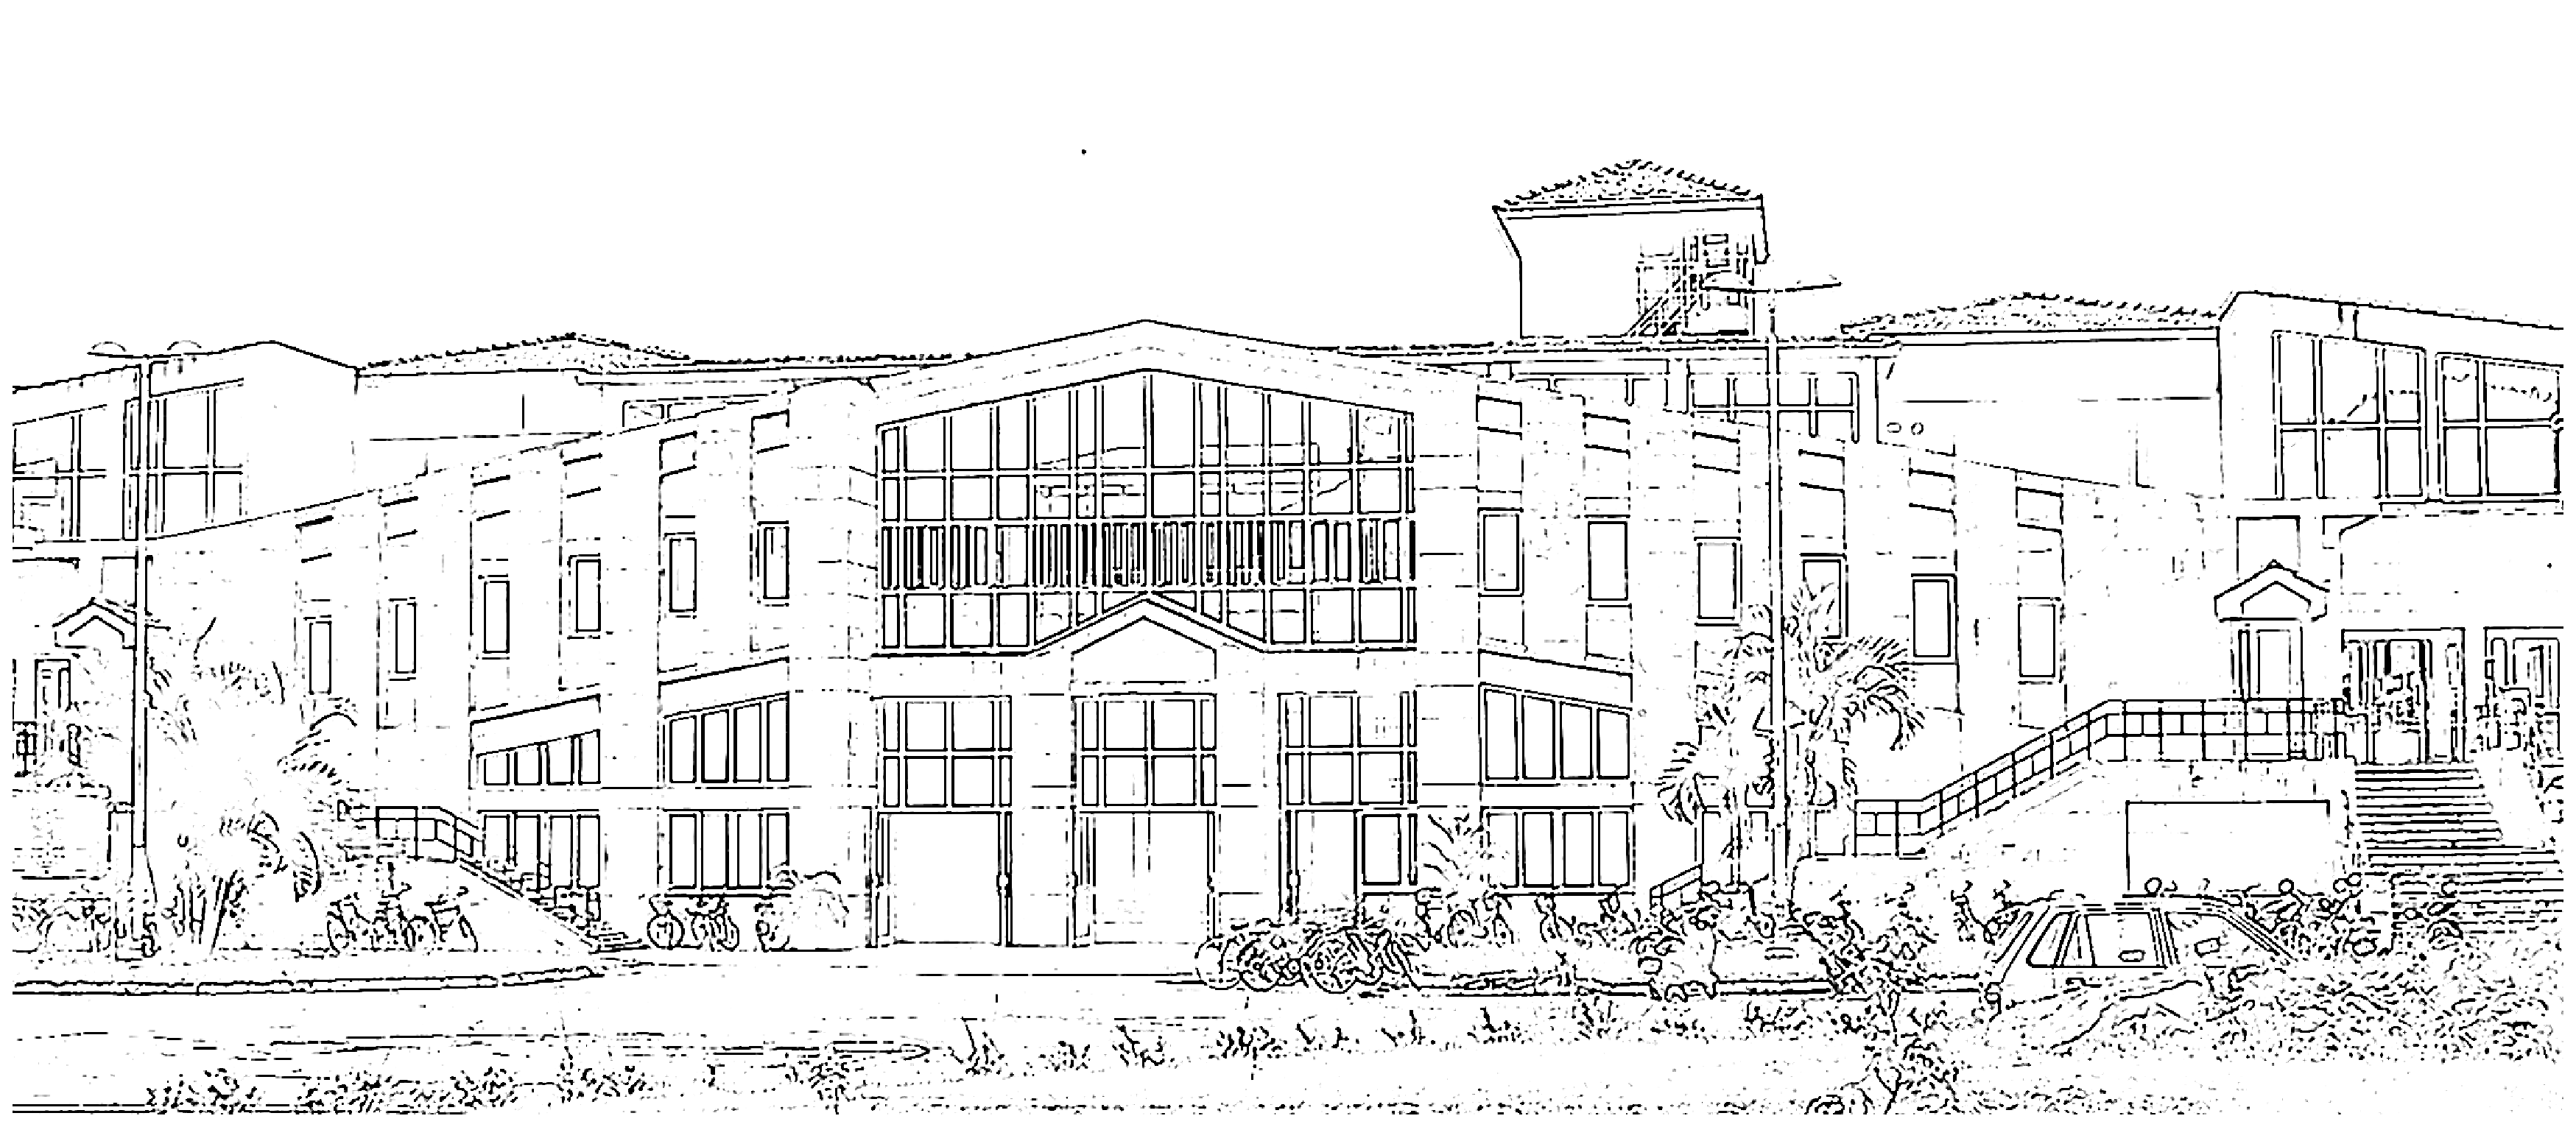
\includegraphics[width=\textwidth]{100-back/academic}
\begin{minipage}{0.2\linewidth}
\includegraphics[width=\textwidth]{100-back/IITG_logo.png}
\end{minipage}
\begin{minipage}{0.78\linewidth}
	\begin{flushleft}
    \textbf{Department of Computer Science and Engineering}\\
    \large{\textbf{Indian Institute of Technology Guwahati}}\\
    \Large{\textbf{Guwahati 781039, India}}
	\end{flushleft}
\end{minipage}
\end{center}

%  \includepdf[pages={4}]{C0_Cover.pdf}
%\printLog
%%%%%%%%%%%%%%%%%%%%%%%%%%%%%%%%%%%%%%%%%%%%%%%%%%%%%%%%%%%%%%%%%
%\jacket
\end{document}
